\documentclass[master=mai,masteroption=ecs,english]{kulemt}
\setup{title={The best master thesis ever},
  author={Een Auteur\and Tweede Auteur},
  promotor={Prof.\,dr.\,ir.\ Weet Beter},
  assessor={Ir.\,W. Eetveel\and W. Eetrest},
  assistant={Ir.\ A.~Assistent \and D.~Vriend}}
% De volgende \setup mag verwijderd worden als geen fiche gewenst is.
\setup{filingcard,
  translatedtitle={Beste masterproef ooit al geschreven},
  udc=621.3,
  shortabstract={Hier komt een heel bondig abstract van hooguit 500
    woorden. \LaTeX\ commando's mogen hier gebruikt worden. Blanco lijnen
    (of het commando \texttt{\string\pa r}) zijn wel niet toegelaten!
    \endgraf \lipsum[2]}}
% Verwijder de "%" op de volgende lijn als je de kaft wil afdrukken
%\setup{coverpageonly}
% Verwijder de "%" op de volgende lijn als je enkel de eerste pagina's wil
% afdrukken en de rest bv. via Word aanmaken.
%\setup{frontpagesonly}

% Kies de fonts voor de gewone tekst, bv. Latin Modern
\setup{font=lm}

% Hier kun je dan nog andere pakketten laden of eigen definities voorzien

% Tenslotte wordt hyperref gebruikt voor pdf bestanden.
% Dit mag verwijderd worden voor de af te drukken versie.
\usepackage[pdfusetitle,colorlinks,plainpages=false]{hyperref}
\usepackage{csquotes}
\usepackage{amsbsy}
\usepackage{outlines}


\newenvironment{myitemize}
{ \begin{itemize}
    \setlength{\itemsep}{0pt}
    \setlength{\parskip}{0pt}
    \setlength{\parsep}{0pt}     }
{ \end{itemize}  }

\newenvironment{myenumerate}
{ \begin{enumerate}
    \setlength{\itemsep}{0pt}
    \setlength{\parskip}{0pt}
    \setlength{\parsep}{0pt}     }
{ \end{enumerate}  }


%%%%%%%
% Om wat tekst te genereren wordt hier het lipsum pakket gebruikt.
% Bij een echte masterproef heb je dit natuurlijk nooit nodig!
\IfFileExists{lipsum.sty}%
 {\usepackage{lipsum}\setlipsumdefault{11-13}}%
 {\newcommand{\lipsum}[1][11-13]{\par Hier komt wat tekst: lipsum ##1.\par}}
%%%%%%%

%\includeonly{chap-n}
\begin{document}

\begin{preface}
  I would like to thank everybody who kept me busy the last year,
  especially my promotor and my assistants. I would also like to thank the
  jury for reading the text. My sincere gratitude also goes to my wive and
  the rest of my family.
\end{preface}

\tableofcontents*

\begin{abstract}
  The \texttt{abstract} environment contains a more extensive overview of
  the work. But it should be limited to one page.

  \lipsum[1]
\end{abstract}

\begin{abstract*}
  In dit \texttt{abstract} environment wordt een al dan niet uitgebreide
  Nederlandse samenvatting van het werk gegeven.
  Wanneer de tekst voor een Nederlandstalige master in het Engels wordt
  geschreven, wordt hier normaal een uitgebreide samenvatting verwacht,
  bijvoorbeeld een tiental bladzijden. 

  \lipsum[1]
\end{abstract*}

% Een lijst van figuren en tabellen is optioneel
%\listoffigures
%\listoftables
% Bij een beperkt aantal figuren en tabellen gebruik je liever het volgende:
\listoffiguresandtables
% De lijst van symbolen is eveneens optioneel.
% Deze lijst moet wel manueel aangemaakt worden, bv. als volgt:
\chapter{List of Abbreviations and Symbols}
\section*{Abbreviations}
\begin{flushleft}
  \renewcommand{\arraystretch}{1.1}
  \begin{tabularx}{\textwidth}{@{}p{12mm}X@{}}
    LoG   & Laplacian-of-Gaussian \\
    MSE   & Mean Square error \\
    PSNR  & Peak Signal-to-Noise ratio \\
  \end{tabularx}
\end{flushleft}
\section*{Symbols}
\begin{flushleft}
  \renewcommand{\arraystretch}{1.1}
  \begin{tabularx}{\textwidth}{@{}p{12mm}X@{}}
    $m$   & Mass \\
    $\pi$ & The number pi \\
    NN  & Neural Network \\
    Item2Vec & Item2Vector \\ 
  \end{tabularx}
\end{flushleft}

 
% Nu begint de eigenlijke tekst
\mainmatter

\chapter{Introduction}
\label{cha:intro}
The first contains a general introduction to the work. The goals are
defined and the modus operandi is explained.

\section{Lorem Ipsum 4--5}
\lipsum[4-5]

\section{Lorem Ipsum 6--7}
\lipsum[6-7]

%%% Local Variables: 
%%% mode: latex
%%% TeX-master: "thesis"
%%% End: 

\chapter{Literature Review}
\label{cha:0}
\lipsum[79]

\section{Word2Vector Models}
The Word2Vector model builds high quality distributed vector representation of words from large corpus of millions of sentences. Each \textbf{word vector} is built from the sets of its context words (words appearing in the same sentence) hence they capture a lot of local semantic and syntactic information useful for several Natural Language Processing tasks. Two different type of models are used for building these word representations as introduced in \cite{Mikolov2013}. They are,
\begin{myitemize}
\item Skip Gram Model
    \begin{myitemize}
    \item \textbf{Training Objective:} Predict the Context words of the Center word
    \end{myitemize}
\item Continuous Bag of Words Model
\begin{myitemize}
    \item \textbf{Training Objective:} Predict the Center word from the Context words. 
    \end{myitemize}
\end{myitemize}

\subsection{Architecture of the Word2Vec Model}
The Item2Vector Neural Network is fully connected two layer Neural Network (One hidden layer and one output layer). The Input to the model is a one hot encoded vector of the center word and the expected output is a one hot encoded vector of the context words. Therefore the size of the input and the output layer is equal to the vocabulary of the corpus. The size of the hidden layer is much smaller than the size of the input/output layer, as we are expecting to learn high quality \textbf{low dimensional} vector representation of words.

\begin{figure}
  \centering
  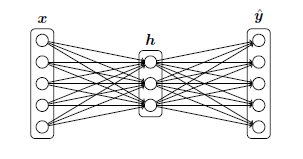
\includegraphics{2_1_NN_Architecture}
  \caption{A Simple Word2Vector Neural Network Architecture}
  \label{fig:1_1_NN_Architecture}
\end{figure}

\fref{fig:1_1_NN_Architecture} shows the architecture of a simple Word2Vector model. Unlike traditional Neural networks, the Word2Vec model does not include biases. It also employs only a linear activation function at the hidden layer. For each word two different distributed vector representations namely \textbf{input vector}  and the \textbf{output vector} are learnt. For example, for the word \textbf{book}, one input vector and one output vector is learnt. The reasons for this becomes obvious when we introduce the output probability estimation equation \ref{eqn:probestimate}. 

\paragraph*{A Description of the notations used in the equations:}
\begin{myitemize}
    \item \textbf{T} be the size of the vocabulary in the training corpus
    \item \textbf{x} be the input to the Neural network
    \item \textbf{N} be the size of the hidden layer
    \item \textbf{$\theta$} be the predicted score at the output layer
    \item \textbf{$\hat{y}$} be the predicted probability of the softmax classifier
    \item \textbf{y} be the true label at the output of the Neural network
    \item \textbf{V} be the weight matrix between the input and the hidden layer. It is of size \textbf{TxN}
    \item \textbf{U} be the weight matrix between the hidden and the output layer. It is of size \textbf{NxT}
\end{myitemize}

\paragraph*{A note on confusing nomenclature}
We can notice that the term input to the Neural network which is the vector \textbf{X} and the the input vector of the $i^{th}$ word \textbf{$u_i$} have the terms input in them. Similarly the output of the Neural network, the vector \textbf{$\theta$} and the output vector of the $j^{th}$ word \textbf{$v_j$} have the terms output in them. I understand that this is very confusing. But to stay consistent with the literature I have retained with this terminology. Each row of \textbf{V} represents the input vector representation of the corresponding word in the input layer and each column of the \textbf{U} represents the output vector representation of the corresponding word in the output layer. 

\fref{fig:1_2_Word2Vec_Architecture} shows the architecture of a simple Word2Vector model \cite{Rong2014}
\begin{figure}
  \centering
  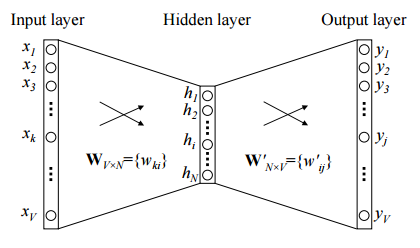
\includegraphics{1_2_Word2Vec_Architecture}
  \caption{A Simple Word2Vector Neural Network Architecture}
  \label{fig:1_2_Word2Vec_Architecture}
\end{figure}

\paragraph*{A Global Overview of modelling process}
Chunks of Math may interrupt the reader from getting a global idea of the whole modelling process. Hence I am presenting the global idea in a nutshell here, hoping that this will aid in better understanding of the following concept.

We are interested in deriving a distributed vector representation of words in our training corpus. For example, consider our training corpus consists of the following three sentences:
\begin{myitemize}
    \item Dog barks at the cat
    \item Cat eats the fish
    \item Caesar was a great king
\end{myitemize}

\begin{myenumerate}
\item Now we take up the first word \textbf{Dog} in the first sentence and encode it as a one hot encoded vector in the vocabulary of the corpus \ref{tab:dogtable}. 
\item Then we take up the words in the context within a window -m to +m and encode them as one hot encoded vector. Here in our case if we consider the context window of size 1, then we take up the word \textbf{barks} alone as context.
\item We propagate the one hot encoded input across the network and estimate the probability of each word in the vocabulary to be its context word.
\item Our training objective is to maximize the log likelihood of the context word given the current word i.e. $\textbf{p(context word|current word)}$ in case of skip-gram and the other way for CBOW.     
\end{myenumerate}

\begin{table}
  \centering
  \begin{tabular}{|c|c|c|c|c|c|c|c|}
  \hline
       Dog&barks&cat&eats&fish&Caesar&great&king  \\
       \hline
       1&0&0&0&0&0&0&0 \\
       \hline
  \end{tabular}
  \caption{One hot encoded vector of the word \textbf{Dog}}
  \label{tab:dogtable}
\end{table}






\subsection{Forward Propagation}
Remember \textbf{x} is the one hot encoded input to the neural network. In the forward propagation, the following computations are performed:

\begin{equation}
    \textbf{h} = \textbf{$v_{i}$}^T \textbf{x}
    \label{eqn:forwardprop1}
\end{equation}

\begin{equation}
    \textbf{$\theta$}=\textbf{$u_{j}$}^T \textbf{h}     
    \label{eqn:forwardprop2}
\end{equation}

We can see that essentially the equations \ref{eqn:forwardprop1} and \ref{eqn:forwardprop1} is just a dot product between the input vector of the $i^{th}$ word and the output vector of the $j^{th}$ word. The resulting \textbf{score} somehow intuitively tells us the un-normalized similarity of these two word vectors.

\subsection{Probability of the Output words}
Once we have computed the similarity scores between the input word and all the other words in the vocabulary, we can estimate the probability of the $j^{th} $ word being the context word when the $i^{th} $ word is the input word using the softmax function as follows:
\begin{equation}
    \hat{y_{ij}}=softmax(v_i*u_j)=softmax(\theta_{ij})
    \label{eqn:probestimate}
\end{equation}

\begin{figure}
  \centering
  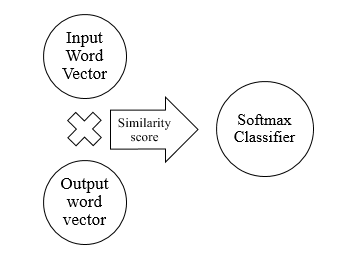
\includegraphics{1_3_Overall_process}
  \caption{Overall Word2Vector Model building process}
  \label{fig:1_3_Overall_process}
\end{figure}


\subsection{Training Objective}
The objective of the training is to maximize the log likelihood of the context word vector given the current word vector. 

\begin{equation}
    \hat{max} J(\theta)=\sum_{-m<j<m,j\neq0}{log(p(w_{c+j}|w_c))}
\end{equation}
\begin{equation}
    =\sum_{-m<j<m,j\neq0}{log(\hat{y}_{c,c+j})}
\end{equation}

\begin{equation}
    =\sum_{-m<j<m,j\neq0}{log(softmax(\theta_{c,c+j}))}
\end{equation}
\begin{equation}
    =\sum_{-m<j<m,j\neq0}{log(softmax(v_{c}^T u_{c+j}))}
    \label{eqn:objective4}
\end{equation}


Equation \ref{eqn:objective4} clearly shows that the objective of the training is to maximize the logarithm of the softmax classifier output, given the context word vector and the current word vector. The figure \ref{fig:1_3_Overall_process} also shows this clearly.

Following this, we have to learn the parameters of the model which will optimize the objective function. Generally Stochastic gradient techniques and Backpropagation algorithm are used for parameter update.

%%% Local Variables: 
%%% mode: latex
%%% TeX-master: "thesis"
%%% End: 

\chapter{Item2Vector Neural Network Architecture}
\label{cha:1}
The success of Neural network models especially the Word2Vector model has been a great inspiration for this Item2Vector model. We see that the distributed vector representation of words has been so powerful in capturing a lot of local information which many other algorithms like Latent Semantic Indexing are not able to capture. One of the most important objectives of this thesis is to similarly develop a \textbf{distributed representation of items} in the corpus so that each user can be represented as a linear combination of the items that he has rated. Thereafter a collaborative filtering based recommendation system can be built in this low-dimensional space.  We accomplish the objective of developing a distributed representation of items in the corpus with a simple two layer Neural network very similar to Word2Vector model which we shall name as Item2Vector model (named after its inspiration). This chapter has the following sections:
\begin{myitemize}
    \item Architecture of the Item2Vector Neural Network
    \begin{myitemize}
        \item Input, Output, Activation Function
    \end{myitemize}
    \item Forward Propagation Algorithm
    \item Loss functions
    \item Parameter Learning
    \begin{myitemize}
         \item Backpropagation Algorithm
        \item Stochastic Gradient descent Algorithm
    \end{myitemize}
\end{myitemize}


We start this chapter by reasoning out the inspiration of this model to the reader, and then introducing the architecture of the Item2Vector Neural network, followed by a discussion of the Forward Propagation algorithm in which the input is propagated  across the hidden layer and the output is estimated.  Later on, we discuss the possible different loss/objective functions which estimates the efficiency of our model. Following this, we discuss the back propagation algorithm and the stochastic gradient descent algorithm to optimize the parameters of the model, consequently optimizing the cost function. 

\section{Reasoning out the inspiration}


\section{Description of the Neural Network Architecture}
\begin{figure}
  \centering
  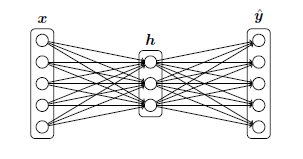
\includegraphics{2_1_NN_Architecture}
  \caption{A Simple Item2Vector Neural Network Architecture}
  \label{fig:2_1_NN_Architecture}
\end{figure}

\fref{fig:2_1_NN_Architecture} The Item2Vector Neural Network is fully connected two layer Neural Network (One hidden layer and one output layer). The size of the hidden layer i.e. the number of hidden neurons, depends upon the data set and the type of application. In general it is preferable to choose the size of the hidden layer using cross validation if regularization parameters have not been employed. In our case the size of the hidden layer is equal to the number of Eigen vectors retained while building the SVD model so that we can have a fair comparison at the end.



\begin{center}
[Twilight Part 1, Twilight Part 2, Twilight Part 3, Twilight Part 4, Twilight Part 5]
\end{center}

In case of Skip-gram model, when an item is given as input called as center item, all the items which usually occur along with it called as co-occuring items are predicted. For example, when Twilight Part 2 is given as input, the co-occuring items Twilight Part 1, 3, 4 and 5 are predicted as output. 

In the case of a CBOW model the reverse is true. For example when Twilight Part 1, 2, 3, 4 are given as input, Twilight Part 5 is predicted. 

\subsection{Input to the Neural Network}
The list of items present in the corpus is referred to as the item list. The input to the Neural network is a one hot encoded vector. The one hot encoding depends on the type of the model employed for generating the Item Vectors. In case of the Skip-gram model, the index of the center item is one-hot encoded in the item list and given as input. Whereas in the case of CBOW model, the indices of the co-occuring items is one-hot encoded and given as input. 

\subsection{Hidden Layer and Activation Function}
Let $\boldsymbol{}$ be the one-hot encoded input vector and $\boldsymbol{W_1}$ and $\boldsymbol{b_1}$ be the matrix of weights and vector of biases connecting the input layer to the hidden layer. In the beginning the weights and biases are initialized to some small random values. During the forward propagation, the hidden layer gets initialized as shown in \ref{eqn:ForwardProp_1} :

\begin{equation} \label{eqn:ForwardProp_1}
h=sigmoid(x W_1+b1)
\end{equation}

\subsection{Output layer and Softmax Function}
Let \^{y} be the output vector and $\boldsymbol{W_2}$ and $\boldsymbol{b_2}$ be the matrix of weights and vector of biases connecting the hidden layer to the output layer. The Output vector is estimated as shown in \ref{eqn:ForwardProp_2}:

\begin{equation} \label{eqn:ForwardProp_2}
\hat{y}=softmax(h W_2+b2)
\end{equation}

\section{Adding more intuitive insight to the Neural Network Architecture}
The Skip-gram model as well as the CBOW model results in two vectors corresponding to each item in the list of items. These vectors are called as input and output vectors. The sigmoid of Weights $W_1$ + bias $b_1$ connecting the input layer and the hidden layer, corresponds to the input vector of each item in the list of items. Similarly the weights $W_2$ summed with the bias $b_2$ connecting the hidden layer and the output layer corresponds to the output vector of each item in the list of items. 

After the training, the sigmoid of the sum of vector of weights from an input neuron to each hidden neuron and the bias is the input vector of the item. 
\begin{center}
$v_i=sigmoid(W_{1i}+b1)$
\end{center}
Here, $v_i$ is the input vector of the $i^{th}$ item. 

Similarly the sum of the vector of the weights from all the hidden neurons to one output neuron corresponds to the output vector of that item.
\begin{center}
$u_i=W_{2i}+b2$
\end{center}

Here, $u_i$ is the input vector of the $i^{th}$ item. 

In case of a Skip-gram model, we want to predict the probability of an item co-occuring with an other item. Therefore the similarity of the input vector of the given item and the output vector of the other item is estimated using a simple dot product and then crunched into probability using a soft-max function.

\begin{equation}
\hat{y_{ij}}=softmax(v_i*u_j)
\end{equation}
Here $\hat{y_{i,j}}$ refers to the probability of the $i^{th}$ item co-occuring with the  $j^{th}$ item.

\section{Training the Neural Network}
Let our Neural Network consists of $nh$ hidden neurons, $D_x$ input neurons each corresponding to one item in the list of items and $D_y$ output neurons each corresponding to one item in the list of items. It can been seen that $D_x=D_y$. Therefore our Neural Network consists of $(D_x+1)*nh + (nh+1)*D_y$ parameters.

\subsection{Loss Functions}
I evaluated the performance of the model while optimizing two types of loss functions. The first one is the cross entropy loss and the second one is negative sampling. 
\subsubsection{Cross Entropy Loss}
Cross entropy loss can be estimated as shown in \ref{eqn:Cross_Entropy}

\begin{equation}
J_{CE}(y,\hat{y})=\sum_{i}^{D_y}y_i log(\hat{y_i})
\label{eqn:Cross_Entropy}
\end{equation}

\begin{equation}
\hat{y_i}=p(i|c)=\frac{exp(u_i^T v_c )}{\sum_{w=1}^{D_y}u_w^T v_c}
\label{y_hat}
\end{equation}

\subsubsection{Negative Sampling Loss Function}
The Negative sampling loss function can be estimated as shown in \ref{eqn:Negative_loss}

\begin{equation}
J_{neg-sample}=-log(\sigma(u_o^T v_c))-\sum_{k=1}^{K} log (-\sigma(u_k^T v_c))
\label{eqn:Negative_loss}
\end{equation}





%%% Local Variables: 
%%% mode: latex
%%% TeX-master: "thesis"
%%% End: 

\chapter{The Next Chapter}
\label{cha:2}
\lipsum[77]

\section{The First Topic of this Chapter}
\lipsum[78]

\subsection{An item}
A master thesis is never an isolated work. This means that your text must
contain references. On-line documents as well as
books can be referenced.

\section{Figures}
Figures are used to add illustrations to the text. The \fref{fig:logo} shows
the KU~Leuven logo as an illustration.
\begin{figure}
  \centering
  
\includegraphics{logokul}
  \caption{The KU~Leuven logo.}
  \label{fig:logo}
\end{figure}

\section{Tables}
Tables are used to present data neatly arranged. A table is normally
not a spreadsheet! Compare \tref{tab:wrong} en \tref{tab:ok}: which table do
you prefer?

\begin{table}
  \centering
  \begin{tabular}{||l|lr||} \hline
    gnats     & gram      & \$13.65 \\ \cline{2-3}
              & each      & .01 \\ \hline
    gnu       & stuffed   & 92.50 \\ \cline{1-1} \cline{3-3}
    emu       &           & 33.33 \\ \hline
    armadillo & frozen    & 8.99 \\ \hline
  \end{tabular}
  \caption{A table with the wrong layout.}
  \label{tab:wrong}
\end{table}

\begin{table}
  \centering
  \begin{tabular}{@{}llr@{}} \toprule
    \multicolumn{2}{c}{Item} \\ \cmidrule(r){1-2}
    Animal    & Description & Price (\$)\\ \midrule
    Gnat      & per gram    & 13.65 \\
              & each        & 0.01 \\
    Gnu       & stuffed     & 92.50 \\
    Emu       & stuffed     & 33.33 \\
    Armadillo & frozen      & 8.99 \\ \bottomrule
  \end{tabular}
  \caption{A table with the correct layout.}
  \label{tab:ok}
\end{table}

\section{Lorem Ipsum}
This section is added to check headers and footers. So this chapter must at
least contain three pages. To make sure that we get the required amount,
the \textsf{lipsum} package isn't used but the text is put directly in the
text.

\subsection{Lorem ipsum dolor sit amet, consectetur adipiscing elit}
Sed nec tortor id felis tristique sodales. Nulla nec massa eu dui fermentum
tincidunt. Integer ullamcorper ante eget eros posuere faucibus. Nam id
ligula ut augue pulvinar vulputate id at purus. Aenean condimentum tortor
eu mi placerat eget eleifend massa mollis. Nam est mi, sagittis quis
euismod eget, sagittis in nibh. Proin elit turpis, aliquam et imperdiet
sed, volutpat eu turpis.

Pellentesque vel enim tellus, vitae egestas turpis. Praesent malesuada elit
non nisi sollicitudin non blandit lacus tincidunt. Morbi blandit urna at
lectus ornare laoreet. Suspendisse turpis diam, lobortis dictum luctus
quis, commodo at lorem. Integer lacinia convallis ultricies. Sed quis augue
neque, eu malesuada arcu. Nullam vehicula, purus vitae sagittis pulvinar,
erat eros semper massa, eu egestas nibh erat quis magna. Cras pellentesque,
nisl eu dapibus volutpat, urna augue ornare quam, quis egestas lectus nulla
a lectus.

Vivamus dictum libero in massa cursus sed vulputate eros imperdiet. Donec
lacinia, libero ac lobortis egestas, nibh dui ornare arcu, luctus porttitor
velit massa sit amet quam. Maecenas scelerisque laoreet diam, vitae congue
quam adipiscing vitae. Aliquam cursus nisl a leo convallis eleifend
fermentum massa porta. Nunc libero quam, dapibus dapibus molestie sit amet,
faucibus vel nunc.

\subsection{Praesent auctor venenatis posuere}
Sed tellus augue, molestie in pulvinar lacinia, dapibus non ipsum. Fusce
vitae mi vitae enim ullamcorper hendrerit eu malesuada est. Proin iaculis
ante sed nibh tincidunt vel interdum libero posuere. Vivamus accumsan metus
quis felis congue suscipit dapibus enim mattis. Fusce mattis tortor eget
ipsum interdum sagittis auctor id metus.

Integer diam lacus, pharetra sit amet tempor et, tristique non lorem.
Aenean auctor, nisi eu interdum fermentum, lectus massa adipiscing elit,
sed facilisis orci odio a lectus. Proin mi nibh, tempus quis porta a,
viverra quis enim. In sollicitudin egestas libero, quis viverra velit
molestie eget. Nulla rhoncus, dolor a mollis vestibulum, lacus elit semper
nisi, nec sollicitudin sem urna eu magna. Nunc sed est urna, euismod congue
mi.

\subsection{Cras vulputate ultricies venenatis}
Vivamus eros urna, sodales accumsan semper vel, lobortis sit amet mauris.
Etiam condimentum eleifend lorem, ullamcorper ornare lectus aliquet vitae.
Praesent massa enim, interdum sit amet semper et, venenatis ut elit.
Quisque faucibus, quam ac lacinia imperdiet, nulla neque elementum purus,
tempus rutrum justo massa porta sapien. Vestibulum ante ipsum primis in
faucibus orci luctus et ultrices posuere cubilia Curae; Sed ultrices
interdum mi, et rhoncus sapien rutrum sed.

Duis elit orci, molestie quis sollicitudin sed, convallis non ante.
Maecenas tincidunt condimentum justo, et ultricies leo tristique vitae.
Vestibulum quis quam non lectus dapibus eleifend a vitae nibh. Nam nibh
justo, pharetra quis iaculis consequat, elementum quis justo. Etiam mollis
lacinia lacus, nec sollicitudin urna lobortis ac. Nulla facilisi.

Proin placerat risus eleifend erat ultricies placerat. Etiam rutrum magna
nec turpis euismod consectetur. Phasellus tortor odio, lacinia imperdiet
condimentum sed, faucibus commodo erat. Phasellus sed felis id ante
placerat ultrices. Aenean tempor justo in tortor volutpat eu auctor dolor
mollis. Aenean sit amet risus urna. Morbi viverra vehicula cursus.

\subsection{Donec nibh ante, consectetur et posuere id, tempus nec arcu}
Curabitur a tellus aliquet ipsum pellentesque scelerisque. Etiam congue,
risus et volutpat rutrum, est purus dapibus leo, non cursus metus felis
eget ligula. Vivamus facilisis tristique turpis, ut pretium lectus luctus
eleifend. Fusce magna sapien, ullamcorper vitae fringilla id, euismod quis
ante.

Phasellus volutpat, nunc et pharetra semper, sem justo adipiscing mauris,
id blandit magna quam et orci. Vestibulum a erat purus, ut molestie ante.
Vestibulum ante ipsum primis in faucibus orci luctus et ultrices posuere
cubilia Curae; Proin turpis diam, consequat ut ullamcorper ut, consequat eu
orci. Sed metus risus, fringilla nec interdum vel, interdum eu nunc.
Suspendisse vel sapien orci.

\subsection{Morbi et mauris tempus purus ornare vehicula}
Mauris sit amet diam quam, eget luctus purus. Sed faucibus, risus semper
eleifend iaculis, mi turpis bibendum nisl, quis cursus nibh nisl sit amet
ipsum. Vestibulum tempor urna vitae mi auctor malesuada eget non ligula.
Nullam convallis, diam vel ultrices auctor, eros eros egestas elit, sed
accumsan arcu tortor eget leo. Vestibulum orci purus, porttitor in pharetra
eget, tincidunt eget nisl. Nullam sit amet nulla dui, facilisis vestibulum
dui.

Donec faucibus facilisis mauris ac cursus. Duis rhoncus quam sed nisi
laoreet eu scelerisque massa tincidunt. Vivamus sit amet libero nec arcu
imperdiet tempor quis non libero. Sed consequat dignissim justo. Phasellus
ullamcorper, velit quis posuere vulputate, felis erat tincidunt mauris, at
vestibulum justo lectus et turpis. Maecenas lacinia convallis euismod.
Quisque egestas fermentum sapien eu dictum. Sed nec lacus in purus dictum
consequat quis vel nisl. Fusce non urna sem. Curabitur eu diam vitae elit
accumsan blandit. Nullam fermentum nunc et leo dictum laoreet. Donec semper
varius velit vel fringilla. Vivamus eu orci nunc.

\section{Conclusion}
The final section of the chapter gives an overview of the important results
of this chapter. This implies that the introductory chapter and the
concluding chapter don't need a conclusion.

\lipsum[66]

%%% Local Variables: 
%%% mode: latex
%%% TeX-master: "thesis"
%%% End: 

% ... en zo verder tot
\chapter{The Final Chapter}
\label{cha:n}
\lipsum[79]

\section{The First Topic of this Chapter}
\subsection{Item 1}
\subsubsection{Sub-item 1}
\lipsum[80]

\subsubsection{Sub-item 2}
\lipsum[81]

\subsection{Item 2}
\lipsum[82]

\section{The Second Topic}
\lipsum[83-85]

\section{Conclusion}
\lipsum[86-88]

%%% Local Variables: 
%%% mode: latex
%%% TeX-master: "thesis"
%%% End: 

\chapter{Conclusion}
\label{cha:conclusion}
The final chapter contains the overall conclusion. It also contains
suggestions for future work and industrial applications.

\lipsum[1-7]

%%% Local Variables: 
%%% mode: latex
%%% TeX-master: "thesis"
%%% End: 


% Indien er bijlagen zijn:
\appendixpage*          % indien gewenst
\appendix
\chapter{The First Appendix}
\label{app:A}
Appendices hold useful data which is not essential to understand the work
done in the master thesis. An example is a (program) source.
An appendix can also have sections as well as figures and references\cite{h2g2}.

\section{More Lorem}
\lipsum[50]

\subsection{Lorem 15--17}
\lipsum[15-17]

\subsection{Lorem 18--19}
\lipsum[18-19]

\section{Lorem 51}
\lipsum[51]

%%% Local Variables: 
%%% mode: latex
%%% TeX-master: "thesis"
%%% End: 

% ... en zo verder tot
\chapter{The Last Appendix}
\label{app:n}
Appendices are numbered with letters, but the sections and subsections use
arabic numerals, as can be seen below.

\section{Lorem 20-24}
\lipsum[20-24]

\section{Lorem 25-27}
\lipsum[25-27]

%%% Local Variables: 
%%% mode: latex
%%% TeX-master: "thesis"
%%% End: 


\backmatter
% Na de bijlagen plaatst men nog de bibliografie.
% Je kan de  standaard "abbrv" bibliografiestijl vervangen door een andere.
\bibliographystyle{abbrv}
\bibliography{library}

\end{document}

%%% Local Variables: 
%%% mode: latex
%%% TeX-master: t
%%% End: 
